\documentclass[11pt]{article}
\usepackage[margin=1.15in]{geometry}
\usepackage{amsmath,amssymb,amsthm}
\usepackage{booktabs,array}
\usepackage[T1]{fontenc}
\usepackage{lmodern}
\usepackage{tikz}
\usetikzlibrary{arrows.meta,positioning}
\usepackage[hidelinks]{hyperref}
\newtheorem{lemma}{Lemma}
\newtheorem{proposition}[lemma]{Proposition}
\newtheorem{corollary}[lemma]{Corollary}
\newtheorem{thm}{Theorem}
\renewcommand{\thethm}{\Alph{thm}}
\theoremstyle{remark}
\newtheorem{remark}[lemma]{Remark}
\newcommand{\norm}[1]{\lVert #1\rVert}
\newcommand{\ML}{\mathrm{ML}}
\newcommand{\loo}{\mathrm{loo}}
\newcommand{\Z}{\mathbb{Z}}
\newcolumntype{L}[1]{>{\raggedright\arraybackslash}p{#1}}
\newcommand{\lab}[1]{\par\smallskip\noindent\textit{Label: #1.}}
\title{Leave-one-out values of tight Goddyn--Wong vectors}
\author{Vico Bonfioli}
\date{31 October 2026. Preprint, not peer reviewed.}
\sloppy\emergencystretch=4em
\begin{document}
\maketitle

\begin{abstract}
For a finite set $W$ of positive integers let $\ML(W)=\max_t\min_{w\in W}\norm{wt}$, where $\norm{x}$ is the distance from $x$ to the nearest integer. A Goddyn--Wong vector is $V=([n-1]\setminus\{r\})\cup\{\mu r\}$ with an integer multiplier $\mu\ge2$; Goddyn and Wong determined when $\ML(V)=1/n$, the value predicted by the lonely runner conjecture for $n-1$ speeds. We determine $\loo(V)=\min_{v\in V}\ML(V\setminus\{v\})$ in three regimes. If $r=n-2$ and $r$ is even and at least $34$, then $\loo(V)=\mu/(\mu r+1)$ for $2\le\mu\le r-1$ (Theorem~A). If $V$ is tight and $n\ge31$, then $\loo(V)=1/(n-1)$ exactly when $\gcd(r,n-1)>1$, and $\loo(V)>1/(n-1)$ otherwise (Theorem~B). If $V$ is tight, $n-r\ge4$, $\gcd(r,n-1)=1$ and $n\ge33$, then $\loo(V)=1/(n-2)$ with a unique minimising deletion (Theorem~C). The proofs are written by hand, rest on two quoted results (the Goddyn--Wong equality criterion and explicit bounds for the prime counting function), and are supported by exact computations for small cases. Nothing is formalized in Lean.
\end{abstract}

\section{Introduction}\label{sec:intro}

\subsection{Setting}
Write $\norm{x}=\operatorname{dist}(x,\Z)$ and, for a finite set $W\subset\Z_{>0}$, $\ML(W)=\max_{t\in\mathbb R}\min_{w\in W}\norm{wt}$. The lonely runner conjecture states $\ML(W)\ge1/(|W|+1)$. A set with $\ML(W)=1/(|W|+1)$ is called \emph{tight}. Goddyn and Wong \cite{GW06} studied the sets $[n-1]_{r\to\mu r}$ obtained from $[n-1]=\{1,\dots,n-1\}$ by replacing the element $r$ by $\mu r$; Theorem~2.3 of \cite{GW06} (restated as Theorem~1.1 of \cite{Zhang26}, where the multiplier is called $m$) is quoted in Section~\ref{sec:imports}. Throughout, the multiplier is called $\mu$ because $m=n-1$ denotes the number of speeds.

\emph{Standing notation.} Integers $n\ge4$, $2\le r\le n-2$, $\mu\ge2$; $s=n-r\ge2$; $V=V(n,r,\mu)=([n-1]\setminus\{r\})\cup\{\mu r\}$; $\loo(V)=\min_{v\in V}\ML(V\setminus\{v\})$. The \emph{Goddyn--Wong condition} is
\begin{equation}\tag{GW}\label{eq:GW}
\gcd(r,b)>1\quad\text{for every integer }b\in[s,\mu s-1].
\end{equation}
By Theorem~2.3 of \cite{GW06}, $\ML(V)\ge1/n$ always, with equality exactly when \eqref{eq:GW} holds (apart from the exceptions $n=2$ and $(n,r,\mu)=(3,1,4)$, which do not meet $n\ge4$). Under \eqref{eq:GW} the set $V$ has $m=n-1$ speeds and is tight. The question of this note is how small $\ML(V\setminus\{v\})$ can be: removing one speed from a tight set leaves a set of $m-1$ speeds, for which the conjectured floor is $1/m$.

\subsection{Labels and provenance}
PROVED: a complete written proof, relative to the imports named in the label, checked step by step by a second session of the same AI system that had not written it; not formalized and not refereed by a human. COMPUTED: an exact finite computation in integer arithmetic whose program is archived; a computed range is a statement about that range only. Where a result depends on an import, its strength is that of the import. Section~\ref{sec:status} lists the checks and the points that were not checked.

The results were obtained with the assistance of an AI system (Claude, Anthropic). The questions and research directions came from the author. The proofs and the computer searches were produced by the AI system; no Lean formalization exists for the results of this note. The author is responsible for all claims.

\subsection{Results}\label{sec:results}
\begin{center}\footnotesize
\begin{tabular}{@{}lL{7.3cm}L{3.6cm}@{}}
\toprule
Item & Statement & Label\\
\midrule
Lemma~\ref{lem:struct} & \eqref{eq:GW} with $\mu,s\ge2$ gives $s\le r-1$ and $\mu s\le r+1$ & PROVED (hand)\\
Lemma~\ref{lem:ub} & $[k-1]\cup\{\mu k\}\subseteq W$ implies $\ML(W)\le\mu/(\mu k+1)$ & PROVED (hand)\\
Cor.~\ref{cor:s2} & $s=2$: $\ML(V\setminus\{n-1\})=\mu/(\mu r+1)$ & PROVED (hand)\\
Lemma~\ref{lem:top} & Under \eqref{eq:GW}: $\ML(V\setminus\{n-1\})=1/(n-1)$ iff $\gcd(r,n-1)>1$ & PROVED over Thm~2.3 of \cite{GW06}\\
Lemma~\ref{lem:windows} & Three prime windows contain at least $3$ or $4$ primes & PROVED over \cite{Dusart10} for $N\ge10^5$; COMPUTED (exact sieve) for $N\le10^7$\\
Lemma~\ref{lem:witness} & Explicit times for all deletions except the top ones & PROVED over Lemma~\ref{lem:windows}\\
Thm~A & $r$ even, $r\ge34$, $n=r+2$, $2\le\mu\le r-1$: $\loo(V)=\mu/(\mu r+1)$, attained at the deletion of $n-1$ & PROVED over Lemma~\ref{lem:windows}; $r\le32$: COMPUTED (240 vectors)\\
Thm~B & \eqref{eq:GW}, $s\ge2$, $n\ge31$: $\loo(V)=1/(n-1)$ iff $\gcd(r,n-1)>1$ (only the deletion of $n-1$ attains it); otherwise $\loo(V)>1/(n-1)$ & PROVED over Thm~2.3 of \cite{GW06} and Lemma~\ref{lem:windows}; $n<31$: COMPUTED\\
Lemma~\ref{lem:coprime}, Prop.~\ref{prop:ub2}, Cor.~\ref{cor:ub2} & Structure of the coprime case; $\ML(V\setminus\{n-2\})=1/(n-2)$ & PROVED over Thm~2.3 of \cite{GW06}\\
Lemma~\ref{lem:D} & Deletion of $n-1$ when $\gcd(r,n-1)=1$, $s\ge4$: $\ML\ge2/(2r+s-1)>1/(n-2)$ & PROVED (hand)\\
Thm~C & \eqref{eq:GW}, $s\ge4$, $\gcd(r,n-1)=1$, $n\ge33$: $\loo(V)=1/(n-2)$, unique minimiser $n-2$ & PROVED over Thm~2.3 of \cite{GW06} and Lemma~\ref{lem:windows}; $n\le300$: three vectors COMPUTED\\
\bottomrule
\end{tabular}
\end{center}
Not claimed: vectors with more than one replaced speed, and the case $s=3$. No Lean formalization exists for any item. Section~\ref{sec:status} separates what is proved by hand, what is computed, and what is imported.

\section{Outline of the proof}\label{sec:outline}

\noindent\textbf{Idea in words.}
In the Goddyn--Wong vector, delete one speed. If $s=2$ and the top speed $n-1$ is deleted, the points $0,t,\dots,rt$ of the circle are pairwise more than $\varepsilon$ apart unless the pair is $(0,rt)$, so the other $r$ arcs are longer than $1-1/(\mu r+1)$, the remaining arc from $0$ to $rt$ is short, and $\mu rt$ lies within $\mu/(\mu r+1)$ of an integer. This is the upper bound. For every other deleted speed $j$ a single explicit time shows that the loss is smaller. For small $j$ take $t=a/q$ with $q$ a prime between $1.5n$ and $2n$ and $aj\equiv1\pmod q$, so all other speeds are at least $2/q$ from an integer. For large $j$ take $t=1/j$, moved by a small amount when $j$ divides $\mu r$. The equality criterion of Goddyn and Wong turns tightness after deleting the top speed into the condition $\gcd(r,n-1)>1$. When $\gcd(r,n-1)=1$ and $s\ge4$ the top deletion is harmless, and the minimum moves to the deletion of $n-2$, where a pigeonhole argument at the near-tight time of $V$ gives the upper bound $1/(n-2)$.


Throughout, $\ML(V\setminus\{j\})\ge c$ is shown by exhibiting a time $t$ with $\norm{xt}\ge c$ for all $x\in V\setminus\{j\}$, and $\ML(V\setminus\{j\})\le c$ by a covering argument valid for every $t$.

\begin{enumerate}
\item \textbf{Structure of \eqref{eq:GW}} (Lemma~\ref{lem:struct}): $s\le r-1$, $\mu s\le r+1$, and the element $\mu r$ exceeds $n-1$. All later estimates use only these inequalities.
\item \textbf{Upper bound by a circle-gap argument} (Lemma~\ref{lem:ub}, Corollary~\ref{cor:s2}): for $s=2$ the deletion of $n-1$ gives exactly $\mu/(\mu r+1)$.
\item \textbf{The top deletion in general} (Lemma~\ref{lem:top}): by the equality criterion of \cite{GW06} applied to $V\setminus\{n-1\}$, $\ML(V\setminus\{n-1\})=1/(n-1)$ iff $\gcd(r,n-1)>1$.
\item \textbf{Prime windows} (Lemma~\ref{lem:windows}): three explicit intervals contain at least $3$ or $4$ primes; a sieve covers $N\le10^7$ and the Dusart bounds cover $N\ge10^5$.
\item \textbf{Witness times for all other deletions} (Lemma~\ref{lem:witness}; Theorem~A, parts (a)--(d)): four cases by the size and divisibility of the deleted speed $j$ (one for $j=\mu r$, one for $j$ above $n/2$ not dividing $\mu r$, one for $j$ above $n/2$ dividing $\mu r$, one for $j\le n/2$ using a prime).
\item \textbf{Assembly} (Theorems~A and~B): take the minimum over deletions.
\item \textbf{Coprime case} (Lemma~\ref{lem:coprime}, Proposition~\ref{prop:ub2}, Lemma~\ref{lem:D}, Theorem~C): for $\gcd(r,n-1)=1$, $s\ge4$ the near-tight time of $V$ forces $\ML(V\setminus\{n-2\})\le1/(n-2)$; the deletion of $n-1$ gives at least $2/(2r+s-1)$; Lemma~\ref{lem:witness} with threshold $1/(n-2)$ handles the rest.
\end{enumerate}

\begin{figure}[h]
\centering
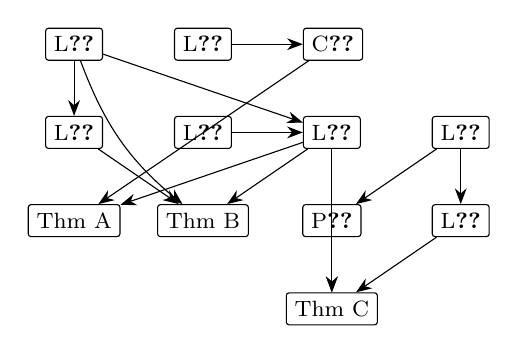
\begin{tikzpicture}[node distance=7mm and 9mm, every node/.style={font=\footnotesize}, box/.style={draw,rounded corners=1pt,inner sep=3pt}, >={Stealth[length=2mm]}]
\node[box] (L1) {L\ref{lem:struct}};
\node[box,right=of L1] (L2) {L\ref{lem:ub}};
\node[box,right=of L2] (C3) {C\ref{cor:s2}};
\node[box,below=of L1] (L4) {L\ref{lem:top}};
\node[box,below=of L2] (L5) {L\ref{lem:windows}};
\node[box,right=of L5] (L6) {L\ref{lem:witness}};
\node[box,below=of L4] (TA) {Thm A};
\node[box,below=of L5] (TB) {Thm B};
\node[box,right=of L6] (L7) {L\ref{lem:coprime}};
\node[box,below=of L6] (P8) {P\ref{prop:ub2}};
\node[box,below=of L7] (L9) {L\ref{lem:D}};
\node[box,below=of P8] (TC) {Thm C};
\draw[->] (L1) -- (L4); \draw[->] (L1) -- (L6); \draw[->] (L2) -- (C3); \draw[->] (C3) -- (TA);
\draw[->] (L5) -- (L6); \draw[->] (L6) -- (TA); \draw[->] (L6) -- (TB); \draw[->] (L4) -- (TB);
\draw[->] (L1) to[bend right=15] (TB);
\draw[->] (L7) -- (P8); \draw[->] (P8) -- (TC); \draw[->] (L9) -- (TC); \draw[->] (L6) -- (TC); \draw[->] (L7) -- (L9);
\end{tikzpicture}
\caption{Dependencies. Theorem~A uses the same witness cases as Lemma~\ref{lem:witness} with thresholds specific to $s=2$ (Section~\ref{sec:A}); the arrow from Lemma~\ref{lem:witness} to Theorem~A records that the case pattern is shared, not a citation of the statement.}
\end{figure}

\section{A worked example}\label{sec:example}

Take $n=8$, $r=6$, $\mu=2$, so $s=2$, $m=7$ and $V=\{1,2,3,4,5,7,12\}$. Condition \eqref{eq:GW} asks $\gcd(6,b)>1$ for $b\in[2,3]$: $\gcd(6,2)=2$ and $\gcd(6,3)=3$. Hence $\ML(V)=1/8$ by (I1) (Section~\ref{sec:imports}); the exact routine gives the same value.

\emph{Deleting $7=n-1$.} The set $W=\{1,2,3,4,5,12\}$ contains $[5]=[k-1]$ with $k=6$ and $\mu k=12$. By Lemma~\ref{lem:ub}, $\ML(W)\le2/13$. At $t^*=2/13$ the residues $jt^*\bmod 1$ for $j=1,\dots,5,12$ are $\tfrac2{13},\tfrac4{13},\tfrac6{13},\tfrac8{13},\tfrac{10}{13},\tfrac{11}{13}$, with distances $\tfrac2{13},\tfrac4{13},\tfrac6{13},\tfrac5{13},\tfrac3{13},\tfrac2{13}$. So $\ML(W)=2/13=\mu/(\mu r+1)$ (Corollary~\ref{cor:s2}).

\emph{The other deletions.} The values are in the table; each is at least $2/13$, and a witness time is given where the proof of Theorem~A supplies one.
\begin{center}\small
\begin{tabular}{@{}rcL{8.6cm}@{}}
\toprule
deleted $j$ & $\ML(V\setminus\{j\})$ & witness\\
\midrule
$1$ & $2/9$ & exact routine ($j\le r/2$; case (d) needs $r\ge34$)\\
$2$ & $2/11$ & exact routine\\
$3$ & $4/17$ & exact routine\\
$4$ & $3/17$ & case (c): $4\mid12$, $d=3$, $t=\tfrac14+\tfrac1{78}=\tfrac{41}{156}$; the distances of $x=1,2,3,5,7,12$ are $\tfrac{41}{156},\tfrac{37}{78},\tfrac{11}{52},\tfrac{49}{156},\tfrac{25}{156},\tfrac2{13}$\\
$5$ & $1/5$ & case (b): $t=\tfrac15$\\
$7$ & $2/13$ & Corollary~\ref{cor:s2}\\
$12$ & $1/6$ & case (a): $t=\tfrac16$\\
\bottomrule
\end{tabular}
\end{center}
Thus $\loo(V)=2/13$, attained only at the deletion of $7$. This agrees with Theorem~A (which is proved for $r\ge34$ and computed for even $r\le32$), and $2/13>1/7$. The script \texttt{code/goddyn-wong-loo/example\_check.py} recomputes every number above in exact arithmetic, with a second computation of $\ML$ over all times $p/q$, $q\le400$.

\emph{A vector with $s=4$.} For $(n,r,\mu)=(74,70,2)$ the condition \eqref{eq:GW} holds ($s=4$, $b\in[4,7]$, and $\gcd(70,b)=2,5,2,7$), $\gcd(70,73)=1$ and this is the first triple of Theorem~C. Here $Q=2r+s-1=143$, $47\cdot70=3290=23\cdot143+1$, so $a=47$, and at $t=47/143$ every $x\in V\setminus\{73\}$ has $\norm{xt}\ge2/143$ (Lemma~\ref{lem:D}); the value $2/143$ is attained at $x=140$ since $140\cdot47\equiv2\pmod{143}$. The exact routine gives $\ML(V\setminus\{72\})=1/72$, $\ML(V\setminus\{73\})=2/143$, $\ML(V\setminus\{140\})=1/70$ and $\loo(V)=1/72$ attained only at $72=n-2$ (file \texttt{data/goddyn-wong-loo/vec\_74\_70\_2.out}).

\section{Imports}\label{sec:imports}

\textbf{(I1) Goddyn--Wong \cite[Theorem~2.3, p.~4]{GW06}.} For $n\ge2$, $r\in[n-1]$ and $m\ge1$, the set $[n-1]_{r\to mr}$ satisfies $\ML\ge1/n$, with equality if and only if $n=2$, or $(n,r,m)=(3,1,4)$, or $\gcd(r,b)>1$ for every $b\in\{n-r,\dots,m(n-r)-1\}$. This is the printed statement (read in the published article; the same statement is Theorem~1.1 of \cite{Zhang26}). The necessity of the gcd condition is proved in \cite{GW06} in the course of the proof of Theorem~2.3 (pp.~4--5); sufficiency is deferred there to Theorem~3.1 of \cite{GW06}. The proof of sufficiency was not read for this note.

\textbf{(I2) Dusart \cite[Theorem~6.9, display (6.6)]{Dusart10}.} $\pi(x)\ge x/(\ln x-1)$ for $x\ge5393$ and $\pi(x)\le x/(\ln x-1.1)$ for $x\ge60184$. The constants and ranges were compared with the printed statement and with a sieve to $2\cdot10^7$ (no violation; both inequalities fail just below the thresholds).

\section{Structure of the condition and the upper bound}\label{sec:basic}

\begin{lemma}\label{lem:struct}
Assume \eqref{eq:GW}, $\mu\ge2$, $s\ge2$. Then (i) $s\le r-1$; (ii) $\mu s\le r+1$, hence $2s\le r+1$ and $\mu\le(r+1)/2$; (iii) $\mu r\ge2r>n-1$, so the $n-1$ speeds of $V$ are distinct and $\mu r$ is the only element of $V$ above $n-1$.
\end{lemma}
\begin{proof}
(i) If $s\ge r$, the interval $[s,\mu s-1]$ contains $(\mu-1)s\ge r$ consecutive integers, hence an integer $b\equiv1\pmod r$, and $\gcd(r,b)=1$, contradicting \eqref{eq:GW}. (ii) By (i), $r+1\ge s$. Since $\gcd(r,r+1)=1$, \eqref{eq:GW} forces $r+1\notin[s,\mu s-1]$, so $b=r+1$, which satisfies $b\ge s$, is not in $[s,\mu s-1]$; that is, $b\ge\mu s$, or $\mu s\le r+1$. With $\mu\ge2$ this gives $2s\le r+1$ and $\mu\le(r+1)/s\le(r+1)/2$. (iii) By (i), $r>s$, so $2r>r+s=n$.
\end{proof}

\begin{lemma}[Upper bound]\label{lem:ub}
Let $k\ge2$, $\mu\ge1$ be integers and $W$ a finite set of positive integers containing $1,\dots,k-1$ and $\mu k$. Then $\ML(W)\le\mu/(\mu k+1)$.
\end{lemma}
\begin{proof}
Put $e=\mu/(\mu k+1)$, so $ke=1-1/(\mu k+1)$. Let $t$ be arbitrary and suppose $\norm{jt}>e$ for $1\le j\le k-1$ and $\norm{\mu kt}>e$. Let $P_i$ be the class of $it$ in $\mathbb R/\Z$, $i=0,\dots,k$. For $i<i'$ with $(i,i')\ne(0,k)$ we have $1\le i'-i\le k-1$, so the circular distance of $P_i,P_{i'}$ is $\norm{(i'-i)t}>e>0$; thus only $P_0$ and $P_k$ may coincide. Order the $k+1$ points cyclically; the $k+1$ arcs between cyclic neighbours have total length $1$, and an arc between neighbours $P,P'$ has length at least their distance.
\emph{Case 1: $P_0$ and $P_k$ are not cyclic neighbours.} Every arc joins a pair other than $(0,k)$, so each exceeds $e$ and the total exceeds $(k+1)e=(k+1)\mu/(\mu k+1)\ge1$, because $(k+1)\mu=\mu k+\mu\ge\mu k+1$. This contradicts the total length $1$.
\emph{Case 2: they are neighbours.} The other $k$ arcs each exceed $e$, so their sum exceeds $ke=1-1/(\mu k+1)$, and the arc $a$ between $P_0$ and $P_k$ satisfies $a<1/(\mu k+1)\le1/3<1/2$. So $a=\norm{kt}$ and $\norm{\mu kt}\le\mu\norm{kt}<\mu/(\mu k+1)=e$, contradicting $\norm{\mu kt}>e$.
So for every $t$ some element of $W$ has distance at most $e$.
\end{proof}

\begin{corollary}\label{cor:s2}
If $s=2$ ($r=n-2$), then $\ML(V\setminus\{n-1\})=\mu/(\mu r+1)$.
\end{corollary}
\begin{proof}
Here $V\setminus\{n-1\}=\{1,\dots,r-1\}\cup\{\mu r\}$, and Lemma~\ref{lem:ub} with $k=r$ gives $\le$. For $\ge$ put $Q=\mu r+1$ and $t^*=\mu/Q$. For $1\le j\le r-1$ the residue of $\mu j$ modulo $Q$ lies in $[\mu,\mu(r-1)]=[\mu,Q-1-\mu]$, so $\norm{jt^*}\ge\mu/Q$. Also $\mu r\cdot\mu=\mu(Q-1)\equiv-\mu\pmod Q$, so $\norm{\mu rt^*}=\mu/Q$ (note $\mu<Q/2$).
\end{proof}

\begin{remark}
For $\mu=2$ and $k=r$, the value $2/(2r+1)$ is the value of $\ML$ for the sets $[M-2]\cup\{2(M-1)\}$ with $M=r+1$, which is known (Section~\ref{sec:attr}).
\end{remark}

\begin{lemma}[The top deletion]\label{lem:top}
Assume \eqref{eq:GW}, $s\ge2$, $\mu\ge2$, $n\ge5$. Then $\ML(V\setminus\{n-1\})=1/(n-1)$ if $\gcd(r,n-1)>1$, and $\ML(V\setminus\{n-1\})>1/(n-1)$ if $\gcd(r,n-1)=1$ (in particular if $s=2$).
\end{lemma}
\begin{proof}
Put $N=n-1\ge4$. Then $V\setminus\{n-1\}=[N-1]_{r\to\mu r}$ with $r\le N-1$ because $s\ge2$. Apply (I1) at $N$ (the exceptions $N=2$ and $(3,1,4)$ do not occur as $N\ge4$): $\ML=1/N$ iff $\gcd(r,b)>1$ for all $b\in[s-1,\mu(s-1)-1]$, and $\ML>1/N$ otherwise. Since $\mu,s\ge2$, $\mu(s-1)-1\ge s-1$, so $s-1$ belongs to this interval, and the interval lies in $\{s-1\}\cup[s,\mu s-1]$ because $\mu(s-1)-1\le\mu s-1$. Given \eqref{eq:GW}, the condition therefore holds iff $\gcd(r,s-1)>1$. Finally $\gcd(r,s-1)=\gcd(r,n-1-r)=\gcd(r,n-1)$, and for $s=2$ this is $\gcd(r,1)=1$.
\end{proof}

\section{Prime windows}\label{sec:windows}

\begin{lemma}\label{lem:windows}
Let $\pi$ be the prime counting function. (a) For $N\ge31$: $\pi(2N-3)-\pi(\lfloor1.5N\rfloor)\ge3$. (b) For $N\ge34$: $\pi(2N)-\pi(\lfloor1.5N\rfloor)\ge4$. (c) For $N\ge33$: $\pi(2N-5)-\pi(\lfloor1.5N\rfloor)\ge3$. Sharpness: (a) fails at $N=29,30$; (b) fails at $N=33$ and at every even $N\le32$ except $24$; (c) fails at $N=28,\dots,32$ (count $2$) and holds with count $3$ at $N=33,34$.
\end{lemma}
\begin{proof}
\emph{Range $N\le10^7$.} An exact sieve to $2\cdot10^7$ (program \texttt{fixchk primes} for (a) and (b); two separate sieves, \texttt{win} and \texttt{review/wit}, for (c)) gives the three statements for all $N$ in the ranges stated, with minimum counts $3$ (at $N=31$ for (a), $N=33$ for (c)) and $4$ for (b) at even $N=34$.
\emph{Range $N\ge10^5$.} Put $L=\ln(1.5N)>11.9$, $A=L-0.7123$, $B=L-1.1$, so $0<B<A<L$. Let $c\in\{3,5\}$ and $X=2N-c\ge5393$, $Y=1.5N\ge60184$. By (I2), $\pi(\lfloor1.5N\rfloor)\le Y/B$. Since $\ln X\le\ln(2N)=L+\ln(4/3)<L+0.2877$, (I2) gives $\pi(X)\ge X/(\ln X-1)\ge X/A$. The count in each window is therefore at least
\[
D=\frac{2N-c}{A}-\frac{1.5N}{B}=\frac{N(0.5L-1.13155)-cB}{AB},
\]
using $2B-1.5A=0.5L-1.13155$. With $AB<L^2$, $0.5L-1.13155>4.8$ and $cB<5L$, we get $D>(4.8N-5L)/L^2>4.8N/L^2-1$ (as $5/L<1$). The function $N/L^2$ is increasing (derivative $(L-2)/L^3>0$) and equals more than $700$ at $N=10^5$, so $D>3300$, and the count, an integer at least $D$, is at least $4$. Windows (a) and (c) correspond to $c=3$ and $c=5$; for (b) use $\pi(2N)\ge\pi(2N-3)$.
The two ranges overlap, so every $N\ge31$, $33$, $34$ respectively is covered.
\end{proof}

\section{Witness times for the other deletions}\label{sec:witness}

For $c\in\{1,2\}$ put $u=n-c$. The case $c=1$ gives the threshold $1/(n-1)$ of Theorem~B; the case $c=2$ gives the threshold $1/(n-2)$ of Theorem~C.

\begin{lemma}\label{lem:witness}
Assume \eqref{eq:GW}, $\mu\ge2$ and one of: (c=1) $s\ge2$, $n\ge31$; (c=2) $s\ge4$, $n\ge33$. Put $u=n-c$. Then $\ML(V\setminus\{j\})>1/u$ for every $j\in V$ with $j\notin\{n-c,\dots,n-1\}$.
\end{lemma}
\begin{proof}
Every such $j$ lies in exactly one of: (R0) $j=\mu r$; (R3) $j\le n/2$; (R2, R4) $n/2<j\le u-1$, $j\ne r$. For each we give $t$ with $\norm{xt}>1/u$ for all $x\in V\setminus\{j\}$. Note $r<u$ since $s>c$.

\emph{(R0) $j=\mu r$, $t=1/r$.} For $x\le r-1$, $\norm{x/r}\ge1/r$. For $r+1\le x\le n-1$, $x\bmod r=x-r\in[1,s-1]$ and $s-1\le r-2$ (Lemma~\ref{lem:struct}), so $\norm{x/r}\ge1/r>1/u$.

\emph{(R2) $n/2<j\le u-1$, $j\nmid\mu r$, $t=1/j$.} Since $2j\ge n+1$, the only multiple of $j$ in $[1,n-1]$ is $j$, and $\mu r$ is not a multiple. So $\norm{x/j}\ge1/j\ge1/(u-1)>1/u$.

\emph{(R4) $n/2<j\le u-1$, $j\mid\mu r$.} \emph{Step 1: $j<r$.} Otherwise $j=r+i$ with $1\le i\le s-2$. With $g=\gcd(j,r)=\gcd(i,r)\le i$, $j\mid\mu r$ gives $(j/g)\mid\mu(r/g)$ and $\gcd(j/g,r/g)=1$, so $(j/g)\mid\mu$ and $j\le g\mu\le(s-2)\mu=\mu s-2\mu\le r+1-4<r<j$, a contradiction. So $d:=\mu r/j$ is an integer with $d\ge\mu+1$. \emph{Step 2.} Put $\theta=1/(2\mu)$, $\eta=(1+\theta)/(u\mu r)$, $t=1/j+\eta$. \emph{Step 3: $x=\mu r$.} $\mu rt=d+(1+\theta)/u$ and $(1+\theta)/u\le(5/4)/u<1/2$, so $\norm{\mu rt}=(1+\theta)/u>1/u$. \emph{Step 4: $x\in V\setminus\{j,\mu r\}$.} Then $1\le x\le n-1<2j$, $x\ne j$, so $x=ej+\rho$ with $e\in\{0,1\}$, $1\le\rho\le j-1$, and $xt\equiv f=\rho/j+x\eta\pmod1$. Now
\[
x\eta\le(n-1)\frac{5/4}{u\cdot2r}=\frac58\cdot\frac{n-1}{u}\cdot\frac1r<\frac{0.65}{r}<\frac1j,
\]
because $(n-1)/u=1$ for $c=1$ and $(n-1)/u\le32/31$ for $c=2$, $n\ge33$, and $j<r$. So $1/j<f<1$ and $\norm{xt}=\min(f,1-f)$. First, $f>1/j>1/u$. Second, if $\rho\le j-2$ then $1-f>2/j-1/j=1/j>1/u$. Third, if $\rho=j-1$ then $x=j-1$ (the other candidate $2j-1\ge n$ exceeds $n-1$), and $1-f=1/j-(j-1)\eta$; we need $(j-1)\eta<1/j-1/u$. Since $(j-1)\eta<j\eta=(1+\theta)/(du)$ and $1/j-1/u=d/(\mu r)-1/u$, it suffices that $\mu r(d+1+\theta)\le d^2u$; as $u>r$ it suffices that $\mu(d+1)+\mu\theta\le d^2$, that is $\mu(d+1)+\tfrac12\le d^2$. Now $d^2-\mu(d+1)=d(d-\mu)-\mu\ge(\mu+1)-\mu=1$ for $d\ge\mu+1$.

\emph{(R3) $j\le n/2$.} By Lemma~\ref{lem:windows}(a) ($c=1$) or (c) ($c=2$), the interval $(\lfloor1.5n\rfloor,2u-1]$ contains at least $3$ primes, all larger than $n$. Both $\mu r-j$ and $\mu r+j$ are positive ($\mu r\ge2r>n$) and less than $n^2$ ($\mu\le(r+1)/2$ by Lemma~\ref{lem:struct}, $r\le n-2$), and a positive integer below $n^2$ has at most one prime divisor above $n$. So at most two window primes divide $\mu r-j$ or $\mu r+j$; choose a window prime $q$ dividing neither. Let $aj\equiv1\pmod q$ and $t=a/q$. For $x\in V\setminus\{j\}$, $\norm{xt}=|xa\bmod q|/q$ with the residue taken in $(-q/2,q/2]$; we show $xa\not\equiv0,\pm1\pmod q$. If $xa\equiv0$ then $q\mid x$: impossible for $x\le n-1<q$, and for $x=\mu r$ it would give $q\mid\mu$ or $q\mid r$, impossible since $q>n>r>\mu$. If $xa\equiv\pm1$ then $x\equiv\pm j\pmod q$. For $x\le n-1$: $x+j\le(n-1)+\lfloor n/2\rfloor=\lfloor1.5n\rfloor-1<q$ and $|x-j|<n<q$, so $x\equiv\pm j$ forces $x=j$, which is deleted. For $x=\mu r$ the choice of $q$ excludes it. So $\norm{xt}\ge2/q\ge2/(2u-1)>1/u$.
\end{proof}

\section{\texorpdfstring{The case $s=2$: Theorem~A}{The case s=2: Theorem A}}\label{sec:A}

\begin{thm}\label{thm:A}
Let $r\ge34$ be even, $2\le\mu\le r-1$, $n=r+2$ (so $s=2$, $m=r+1$) and $V=\{1,\dots,r-1\}\cup\{r+1,\mu r\}$. Then $\loo(V)=\mu/(\mu r+1)$, attained at the deletion of $r+1=n-1$. Uniqueness of the minimiser is not claimed. For even $r\le32$ and $2\le\mu\le r-1$ (240 vectors) the same value, with unique minimiser $r+1$, is COMPUTED.
\end{thm}
\begin{proof}
The condition \eqref{eq:GW} is not used. Put $Q=\mu r+1$, $c=\mu/Q=1/r-\delta$ with $\delta=1/(rQ)$. Corollary~\ref{cor:s2} gives $\ML(V\setminus\{r+1\})=c$. It remains to show $\ML(V\setminus\{j\})\ge c$ for every other $j\in V$; note $\mu r\ge2r>r+1$. Four cases cover $j=\mu r$ and $j\le r-1$.

\emph{(a) $j=\mu r$, $t=1/r$.} The elements $1,\dots,r-1,r+1$ have $\norm{x/r}\ge1/r>c$.

\emph{(b) $r/2<j\le r-1$, $j\nmid\mu r$, $t=1/j$.} As $r$ is even, $2j\ge r+2>r+1$, so the only multiple of $j$ among the elements $\le r+1$ is $j$; $\mu r$ is not a multiple. So $\norm{x/j}\ge1/j>1/r>c$.

\emph{(c) $r/2<j\le r-1$, $j\mid\mu r$.} Put $d=\mu r/j\ge\mu+1$ (as $j<r$) and $t=1/j+\delta$. For $x=\mu r$: $\mu rt=d+\mu/Q$, so $\norm{\mu rt}=c$. For the other $x\in V\setminus\{j\}$ we have $x\le r+1<2j$ and $x\delta\le(r+1)\delta<1/j$ (as $j(r+1)\le r^2-1<rQ$). Write $x=ej+\rho$ with $e\in\{0,1\}$, $1\le\rho\le j-1$ and $f=\rho/j+x\delta\in(1/j,1)$, so $\norm{xt}=\min(f,1-f)$; $f>1/j>c$. If $\rho\le j-2$ then $1-f>1/j>c$. If $\rho=j-1$, then $x=j-1$, or $x=2j-1$; the latter lies in $V$ only if $2j-1\le r+1$, which with $j>r/2$ forces $j=r/2+1$ and $x=r+1$ (if $2j-1>r+1$ it is not in $V$, because the only element of $V$ above $r+1$ is the multiple $\mu r$ of $j$, while $2j-1\equiv-1\pmod j$ and $j\ge2$). For $x=j-1$: $1-f=1/j-(j-1)\delta\ge c=1/r-\delta$ iff $(j-2)\delta\le(r-j)/(jr)$ iff $j(j-2)\le Q(r-j)$. With $j=\mu r/d$ and $d\ge\mu+1$: $j(j-2)<j^2=\mu^2r^2/d^2\le\mu r^2/d$ and $Q(r-j)=Qr(d-\mu)/d\ge Qr/d>\mu r^2/d$. For $j=r/2+1$, $x=r+1$: $1-f=1/j-(r+1)\delta\ge1/r-\delta$ iff $r\delta\le1/j-1/r=(r-2)/(r(r+2))$ iff $1/Q\le(r-2)/(r(r+2))$. As $Q\ge2r+1$ it suffices that $r(r+2)\le2r^2-3r-2$, that is $r^2-5r-2\ge0$, true for $r\ge6$. So $\norm{xt}\ge c$ for all $x$.

\emph{(d) $1\le j\le r/2$.} By Lemma~\ref{lem:windows}(b) the interval $(1.5r,2r]$ contains at least $4$ primes ($r\ge34$), each larger than $r$. Choose a prime $q$ there with $q\nmid\mu r-j$, $q\nmid\mu r+j$ and $q\ne r+j+1$. This is possible: $\mu r\pm j$ are positive and less than $r^2$ ($\mu\le r-1$), so each has at most one prime divisor above $r$, and at most three window primes are excluded. Let $aj\equiv1\pmod q$, $t=a/q$. For $x\in V\setminus\{j\}$: $xa\equiv0$ needs $q\mid x$, impossible for $x\le r+1<q$, and for $x=\mu r$ it needs $q\mid\mu$ or $q\mid r$, impossible as $q>r>\mu$. If $xa\equiv\pm1$ then $x\equiv\pm j\pmod q$. For $x\le r+1$, $|x-j|<q$, so $x\equiv j$ forces $x=j$ (deleted); $x\equiv-j$ needs $q\mid x+j$ with $0<x+j\le r+1+r/2\le q$, so $x+j=q$, $x=q-j\ge1.5r+1-r/2=r+1$, hence $x=r+1$ and $q=r+j+1$, excluded. For $x=\mu r$ the choice of $q$ excludes it. So $\norm{xt}\ge2/q\ge1/r>c$.

The finite range $r\le32$ is the computation \texttt{loo\_tables thmA}.
\end{proof}

\begin{remark}
For $s=2$, \eqref{eq:GW} says $\gcd(r,b)>1$ for $b\in[2,2\mu-1]$, equivalent to: every prime $\le2\mu-1$ divides $r$. So $\mu=2$ needs $6\mid r$, and $\mu\ge3$ needs $30\mid r$. With $m=r+1$ speeds, $\mu/(\mu r+1)>2/(2m-1)=2/(2r+1)$ if and only if $\mu\ge3$.
\end{remark}

\section{\texorpdfstring{The dichotomy: Theorem~B}{The dichotomy: Theorem B}}\label{sec:B}

\begin{thm}\label{thm:B}
Assume \eqref{eq:GW}, $s\ge2$, $\mu\ge2$, $n\ge31$. If $\gcd(r,n-1)>1$ then $\loo(V)=1/(n-1)$, attained only at the deletion of $n-1$. If $\gcd(r,n-1)=1$ then $\loo(V)>1/(n-1)$.
\end{thm}
\begin{proof}
Lemma~\ref{lem:witness} with $c=1$ (the deletions of $j\ne n-1$ exceed $1/(n-1)$) and Lemma~\ref{lem:top} for $j=n-1$; take the minimum.
\end{proof}

For $n<31$, enumeration of \eqref{eq:GW} with $\mu\ge2$ (all $n\le160$) gives exactly four triples, $(n,r,\mu)=(8,6,2),(14,12,2),(20,18,2),(26,24,2)$, all with $s=2$ and $\gcd(r,n-1)=1$; $\loo=2/13,2/25,2/37,2/49$, equal to $\mu/(\mu r+1)$ (COMPUTED). On all $38$ triples with $n\le160$ the dichotomy of Theorem~B and the values of Theorem~A hold (COMPUTED, \texttt{data/goddyn-wong-loo/loo\_gw160.log}): for example $\loo(V)=\mu/(\mu(m-1)+1)$ for $\mu=2$, $r=6,12,\dots,60$ and for $\mu=3$, $r=30,60,\dots,150$.

\section{\texorpdfstring{The coprime case with $s\ge4$: Theorem~C}{The coprime case with s>=4: Theorem C}}\label{sec:C}

Write $q=n-2$ throughout this section.

\begin{lemma}\label{lem:coprime}
Assume \eqref{eq:GW}, $\mu\ge2$, $s\ge4$, $\gcd(r,n-1)=1$. Then $r$, $s$ and $q$ are even, $\gcd(r,q)\ge2$ and $r>q/2$.
\end{lemma}
\begin{proof}
Since $s\ge4$ and $\mu\ge2$, $[s,2s-1]\subseteq[s,\mu s-1]$, and this interval contains a power of $2$ that is at least $4$; $\gcd(r,2^k)>1$ forces $r$ even. As $\gcd(r,s-1)=\gcd(r,n-1)=1$ and $r$ is even, $s-1$ is odd, so $s$ is even and $q=r+s-2$ is even; thus $\gcd(r,q)\ge2$. Lemma~\ref{lem:struct}(ii) gives $2s\le r+1$, so $q=r+s-2\le(3r-3)/2<2r$.
\end{proof}

\begin{proposition}[Upper bound at the deletion of $n-2$]\label{prop:ub2}
Assume \eqref{eq:GW}, $\mu\ge2$, $s\ge4$, $r>q/2$ and $\gcd(r,q)>1$. Then $\ML(V\setminus\{q\})\le1/q$.
\end{proposition}
\begin{proof}
Put $W=V\setminus\{q\}$ ($q\in V$ as $q\ne r$). Fix $t$. By (I1), $\ML(V)=1/n$, a maximum over $t$, so some $x\in V$ has $\norm{xt}\le1/n$. If $x\ne q$, then $x\in W$ and $1/n<1/q$. Otherwise $\norm{qt}\le1/n$: let $a$ be the nearest integer to $qt$ and $\varepsilon=qt-a$, so $|\varepsilon|\le1/n$ and $t=(a+\varepsilon)/q$. Let $g=\gcd(|a|,q)$ ($g=q$ if $a=0$).
\emph{$g\ge2$.} Put $x=q/g\le q/2<r$. Then $x\in W$ ($x\ne q$, $x\ne r$, $x\ne\mu r$ since $\mu r>n-1$), and $xt=a/g+\varepsilon/g$ with $a/g$ an integer, so $\norm{xt}\le|\varepsilon|/g\le1/(ng)<1/q$.
\emph{$g=1$.} Let $b\in[1,q-1]$ with $ab\equiv1\pmod q$. If $\varepsilon\le0$ then $bt\equiv(1+b\varepsilon)/q\pmod1$ with $0<1+b\varepsilon\le1$ (as $b<q<n$ and $|\varepsilon|\le1/n$), so $\norm{bt}\le1/q$. If $\varepsilon\ge0$ use $q-b$: $(q-b)t\equiv(-1+(q-b)\varepsilon)/q$ with numerator in $[-1,0)$, so $\norm{(q-b)t}\le1/q$. Both $b$ and $q-b$ are units modulo $q$ in $[1,q-1]$; $r$ is not a unit modulo $q$, so neither equals $r$; neither equals $q$ or $\mu r>n-1$. The chosen one therefore lies in $W$ (and $b\ne q-b$ since $q>2$ is even and $b$ is a unit).
In every case some element of $W$ has $\norm{xt}\le1/q$.
\end{proof}

\begin{corollary}\label{cor:ub2}
In the situation of Lemma~\ref{lem:coprime}, $\ML(V\setminus\{n-2\})=1/(n-2)$.
\end{corollary}
\begin{proof}
$\le$ is Lemma~\ref{lem:coprime} with Proposition~\ref{prop:ub2}. For $\ge$ take $t=1/q$: elements $x\le n-3$ are not multiples of $q$, so $\norm{x/q}\ge1/q$; $x=n-1$ gives $\norm{(q+1)/q}=1/q$; for $x=\mu r$, $q\mid\mu r$ would give, with $g=\gcd(q,r)$ dividing $q-r=s-2$, that $q/g$ divides $\mu$ (as $\gcd(q/g,r/g)=1$), so $q\le g\mu\le(s-2)\mu\le r-3<q$, which is false.
\end{proof}

\begin{lemma}[The deletion of $n-1$]\label{lem:D}
Assume \eqref{eq:GW}, $\mu\ge2$, $s\ge4$, $\gcd(r,n-1)=1$. With $Q=2r+s-1$: $\ML(V\setminus\{n-1\})\ge2/Q>1/(n-2)$.
\end{lemma}
\begin{proof}
$\gcd(r,Q)=\gcd(r,s-1)=\gcd(r,n-1)=1$. Take $a$ with $ar\equiv1\pmod Q$ and $t=a/Q$. For $x\in[1,n-2]\setminus\{r\}$ we have $x<Q$, so $xa\not\equiv0$; $xa\equiv1$ iff $x=r$ (deleted); $xa\equiv-1$ iff $x=Q-r=r+s-1=n-1$ (deleted). Hence $\norm{xt}\ge2/Q$. For $x=\mu r$: $xa\equiv\mu\pmod Q$ and $2\le\mu\le(r+1)/s<Q/2$, so $\norm{xt}=\mu/Q\ge2/Q$. Finally $2/Q>1/(n-2)$ iff $2(n-2)>2n-s-1$ iff $s>3$.
\end{proof}

\begin{thm}\label{thm:C}
Assume \eqref{eq:GW}, $\mu\ge2$, $s\ge4$, $\gcd(r,n-1)=1$ and $n\ge33$. Then $\loo(V)=1/(n-2)$, $\ML(V\setminus\{n-2\})=1/(n-2)$, and $\ML(V\setminus\{j\})>1/(n-2)$ for every other $j\in V$; the minimiser is unique.
\end{thm}
\begin{proof}
Lemma~\ref{lem:coprime} and Corollary~\ref{cor:ub2} give $\ML(V\setminus\{n-2\})=1/(n-2)$. Lemma~\ref{lem:D} gives $\ML(V\setminus\{n-1\})>1/(n-2)$. Lemma~\ref{lem:witness} with $c=2$ gives the remaining $j$. Take the minimum.
\end{proof}

\begin{remark}
The threshold $n\ge33$ comes only from the prime window (Lemma~\ref{lem:windows}(c) fails at $n=32$); it is vacuous in practice, because the smallest triple in the case of Theorem~C is $(n,r,\mu)=(74,70,2)$. There are $13$ triples with $n\le1100$, namely $n=74,144,284,354,468,494,564,704,774,866,914,930,984$ (all $\mu=2$; $s=4$ except $s=6$ at $n=468,930$ and $s=8$ at $n=866$), listed by \texttt{enum\_coprime\_case.py}. The case $s=3$ is not covered: $2/Q>1/(n-2)$ fails at $s=3$. For $s=2$ the value is given by Theorem~A.
\end{remark}

\section{Status of the evidence}\label{sec:status}

\textbf{By hand.} Lemmas~\ref{lem:struct}--\ref{lem:top}, \ref{lem:witness}, \ref{lem:coprime}, \ref{lem:D}, Proposition~\ref{prop:ub2}, Corollaries~\ref{cor:s2}, \ref{cor:ub2} and Theorems~A, B, C have written proofs in this note. The proofs were checked step by step by a second AI session that had not written them: the first check (Lemmas~\ref{lem:struct}--\ref{lem:witness} with $c=1$, Theorems~A and~B) found four defects in the write-up (an unproved inequality $s\le r+1$, the number of primes required, a muddled case list, a citation for the prime bounds), all repaired; the second check (Section~\ref{sec:C}) found four defects in the write-up (a bound on $x\eta$ valid only for $u=n-1$, the right end of the prime window, the status of the threshold $n\ge33$, the definition of $a$), all repaired. Neither check found a false statement; thresholds were adjusted during the checks (for example, the number of primes needed in Theorem~A and the right end of the window of Lemma~\ref{lem:windows}(c)). The unified statement of Lemma~\ref{lem:witness} for $c=1,2$, and Lemma~\ref{lem:windows}, which merges three windows, were assembled from the two reviewed proofs for this note. A third AI session re-derived both unified statements, recounted the primes in every window for $N\le10^6$ with its own sieve, and re-ran exact witness checks (about $4.8\cdot10^7$ instances for $c=1$ and $3.3\cdot10^7$ for $c=2$) on 31 October 2026, and found no defect in the mathematics; no human has reviewed them.

\textbf{Exact computation.} All $\ML$ values come from one routine (\texttt{mlcore.rs}: exact, every numerator $k$ of $k/(v_i+v_j)$), whose six control values pass in \texttt{loo\_tables selftest}.
\begin{center}\small
\begin{tabular}{@{}L{5.6cm}L{6.1cm}@{}}
\toprule
Computation & Result\\
\midrule
Prime windows, $N\le10^7$ & Lemma~\ref{lem:windows}(a), (b), (c) and sharpness data; two independent sieves for (c)\\
Prime-counting inequalities of \cite{Dusart10} against a sieve to $2\cdot10^7$ & $0$ violations; both fail just below the thresholds\\
Theorem~A, even $r\le32$, $2\le\mu\le r-1$ & $240$ vectors, all deletions, $\loo=\mu/(\mu r+1)$, unique minimiser $r+1$\\
Theorem~A witnesses, even $r\in[34,160]$, $\mu\le r-1$ & $677120$ removals, $0$ failures (supports the algebra of the proof)\\
Lemma~\ref{lem:witness}, $c=1$, $n\in[31,140]$, $\mu s\le r+1$ & $2122585$ removals, $0$ failures\\
Lemma~\ref{lem:witness}, $c=2$ and Lemma~\ref{lem:D}, $n\in[33,260]$, $\mu\le12$ (synthetic: all $(n,r,\mu)$ with $s\ge4$, $\mu s\le r+1$, $\gcd(r,n-1)=1$) & $29260$ triples, $5272627$ deletions, $0$ failures; a second program on $\mu\le20$: $9613877$ checks, $0$ failures\\
All triples of \eqref{eq:GW} with $\mu\ge2$, $n\le160$ & $38$ triples, all deletions: the dichotomy of Theorem~B and the values of Theorem~A hold; the triples $(74,70,2)$, $(144,140,2)$ have $\loo=1/(n-2)$\\
Coprime case, $n\in[33,300]$, $\mu\le12$ & exactly three triples $(74,70,2)$, $(144,140,2)$, $(284,280,2)$: $\ML(V)=1/n$, $\loo=1/(n-2)$ with unique minimiser $n-2$, second smallest the deletion of $n-1$ (ratios $1.0070$, $1.0035$, $1.0018$); two controls with $\gcd(r,n-1)>1$, $(214,210,2)$ and $(215,210,2)$, give $\loo=1/(n-1)$\\
\bottomrule
\end{tabular}
\end{center}
The synthetic witness checks test the algebra of the explicit times, not the theorems, and the set of genuine triples in the coprime case is small, so the numerics there support the proof without testing it. A table of larger vectors ($n\le1100$) computed by a faster routine is not archived and is not used by any statement.

\textbf{Imports.} (I1) defines the class of vectors in Lemma~\ref{lem:struct}, and is used in Lemma~\ref{lem:top} (both directions) and in Proposition~\ref{prop:ub2} (tightness $\ML(V)=1/n$). (I2) is used only in Lemma~\ref{lem:windows}. The theorems are PROVED relative to these two statements as printed in \cite{GW06} and \cite{Dusart10}; neither proof was re-derived. For (I1) the sufficiency proof in \cite{GW06} was not read.

\textbf{Not Lean.} No result of this note has a Lean statement. Formalization of Lemma~\ref{lem:ub}, Corollary~\ref{cor:s2}, Proposition~\ref{prop:ub2} and Lemma~\ref{lem:D} would need no analysis; Lemma~\ref{lem:windows} needs prime-counting bounds in a proof assistant. None of this was attempted.

\textbf{Not covered.} Vectors in which more than one element is replaced, and the case $s=3$ with $\gcd(r,n-1)=1$ if it occurs, are not treated. No general lower bound for $\loo$ of tight sets is claimed; the obstruction note in this archive records the values for $70$ tight vectors and a conjectured bound, consistent with Theorems~A--C where they apply (the comparison was not repeated here).

\section{Attribution and prior art}\label{sec:attr}

\begin{center}\footnotesize
\begin{tabular}{@{}L{3.3cm}L{1.9cm}L{6.1cm}@{}}
\toprule
Item & Status & Reference location\\
\midrule
Equality criterion \eqref{eq:GW}, $\ML(V)\ge1/n$ & known & \cite[Thm.~2.3, p.~4]{GW06}; restated as \cite[Thm.~1.1]{Zhang26}\\
Lemma~\ref{lem:ub} & no earlier statement located & the case $\mu=2$, $W=[k-1]\cup\{2k\}$ gives the value $2/(2k+1)$ of the known sets $[M-2]\cup\{2(M-1)\}$ \cite[Thm.~5.1]{Kravitz21}, as recorded in the obstruction note; \cite{Kravitz21} was read only at the abstract page\\
Cor.~\ref{cor:s2} & known for $\mu=2$; otherwise as above & as above\\
Lemma~\ref{lem:top} & ours (deduction) & application of \cite[Thm.~2.3]{GW06} at $N=n-1$\\
Lemma~\ref{lem:windows} & standard method; bounds known & bounds from \cite[Thm.~6.9]{Dusart10}; sieve ours\\
Device $t=a/q$, $aj\equiv1\pmod q$ & known device & a similar construction in \cite[Thm.~2.9]{Zhang26} (as read)\\
Lemmas~\ref{lem:witness}, \ref{lem:D}, Thms~A, B, C & ours as stated & no statement on leave-one-out values of Goddyn--Wong vectors located in \cite{Zhang26} (text searched); the obstruction note of this archive records that none was located in \cite{GK25}, \cite{BE26}, \cite{Zhang26} as read; no web search was made for this note\\
Context: tight vectors and finiteness & known & Beck and Everett \cite{BE26}, Giri and Kravitz \cite{GK25}; relevant to the descent question of the obstruction note; no statement of this note is taken from them\\
\bottomrule
\end{tabular}
\end{center}

\bibliographystyle{plain}
\bibliography{refs}

\end{document}
